%% =====================================================================================
%% Overview figure (figure*, text width). Drawn by analysis/overview.py from the counts in
%% tables/num_selfplay.tex; placed right after \label{sec:intro} so it floats to page 2.
%% =====================================================================================
\begin{figure*}[t]
\centering
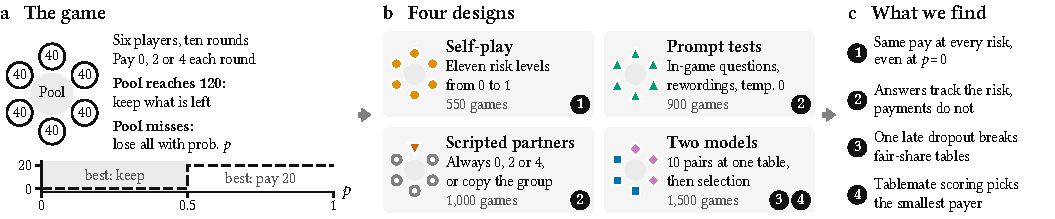
\includegraphics[width=\textwidth]{figures/fig_overview.pdf}
\Description{A three-part overview read from left to right. First, the game: six seats, each
holding 40 units, sit around a shared pool; each round a seat pays 0, 2 or 4, and a small
step plot shows that the best total per seat is 0 below catastrophe probability one half and
20 above it. Second, four design cards, each with a small table of model markers and a game
count: self-play on eleven risk levels, prompt tests, one model beside scripted partners, and
two models at one table followed by selection. Third, four numbered findings that match
numbered badges on the cards.}
\caption{Overview. (a)~Six players hold 40 units and pay 0, 2 or 4 into a shared pool in each
of ten rounds; if the pool misses 120, all savings are lost with probability $p$. Below: the
best total per seat (Proposition~\ref{prop:eq}). (b)~The designs, who sits at each table, and
the number of games. (c)~The findings; badges mark the design behind each.}
\label{fig:overview}
\end{figure*}
